\subsection{Simulator}

The simulator is the main component of the system, it reads the initial configuration and works as a controller between the Petri net engine and the 3D engine.

In order to implement this, we will use the Observer pattern (Figure \ref{fig:observer-pattern}) so that the Simulator can keep track and receive notifications from the 3D engine when some events happen, such as an animation finished or a user interaction.

\begin{figure}[htp]
\begin{center}
  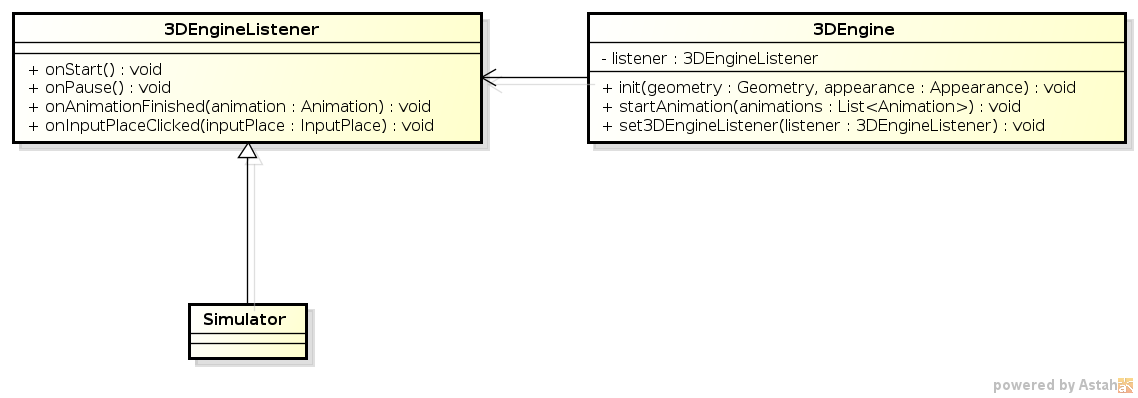
\includegraphics[width=0.8\textwidth]{image/ObserverPattern.png}
  \caption{Simulator with the Observer Pattern}
  \label{fig:observer-pattern}
\end{center}
\end{figure}

Figure \ref{fig:sd-engines} shows the interaction between the three components involved. The simulator starts by reading the configuration, and initializing the Petri net engine with the initial Petri net model as well as the 3D engine with the geometry and the appearance. 

\begin{figure}[htp]
\begin{center}
  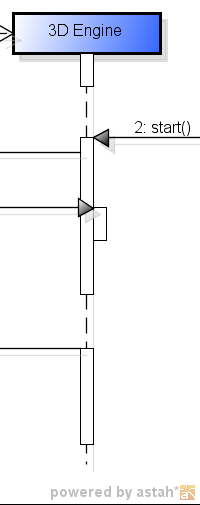
\includegraphics[width=0.8\textwidth]{image/sd-engines.png}
  \caption{Sequence diagram of the Simulator, Petri net Engine and 3D engine}
  \label{fig:sd-engines}
\end{center}
\end{figure}

Then, the 3D engine tells the Simulator that has received a \textit{start simulation} input from the user, and thus, awaits for new animations to be played. The simulator asks the Petri net engine to fire transitions and to give back the next sequence of animations to be played by the 3D engine.